\chapter{Models} \label{ch:models}
This chapter describes the point clouds that will be used as input data to develop and test registration algorithms in the next chapters.

\section{``Hôtel de Ville'' scanning project}
This is a current 3D documentation project by the Image research unit of the \emph{Laboratories of Image, Signal processing and Acoustics} (LISA) at ULB. The goal is to create a full 3D model of the ``Hôtel de Ville de Bruxelles'' \footnote{Brussels Town Hall}. It is a medieval building built in the beginning of the 15th century, with a brabantine gothic-style architecture.

The data set consists of colorized range image point clouds, including both long range and short range scans. Figure \ref{fig:scan_005} shows one of the long-range scans depicting the front facade. It has a complex shape, and contains stone sculptures and other artwork of which close range scans have also been made. The figure depicts a reprojection of a colorized point cloud, where the virtual camera position was set so as to produce a frontal view of the facade. The scan was taken with the scanner placed on the ground, at the left side near the front gate. As a result, points at higher altitudes, such as on the tower, are less densely distributed. Figure \ref{fig:hdv_033_color} from chapter \ref{ch:theory} also shows one of the long-range scans, taken from the roof of the building.

\begin{figure}[h]
\centering
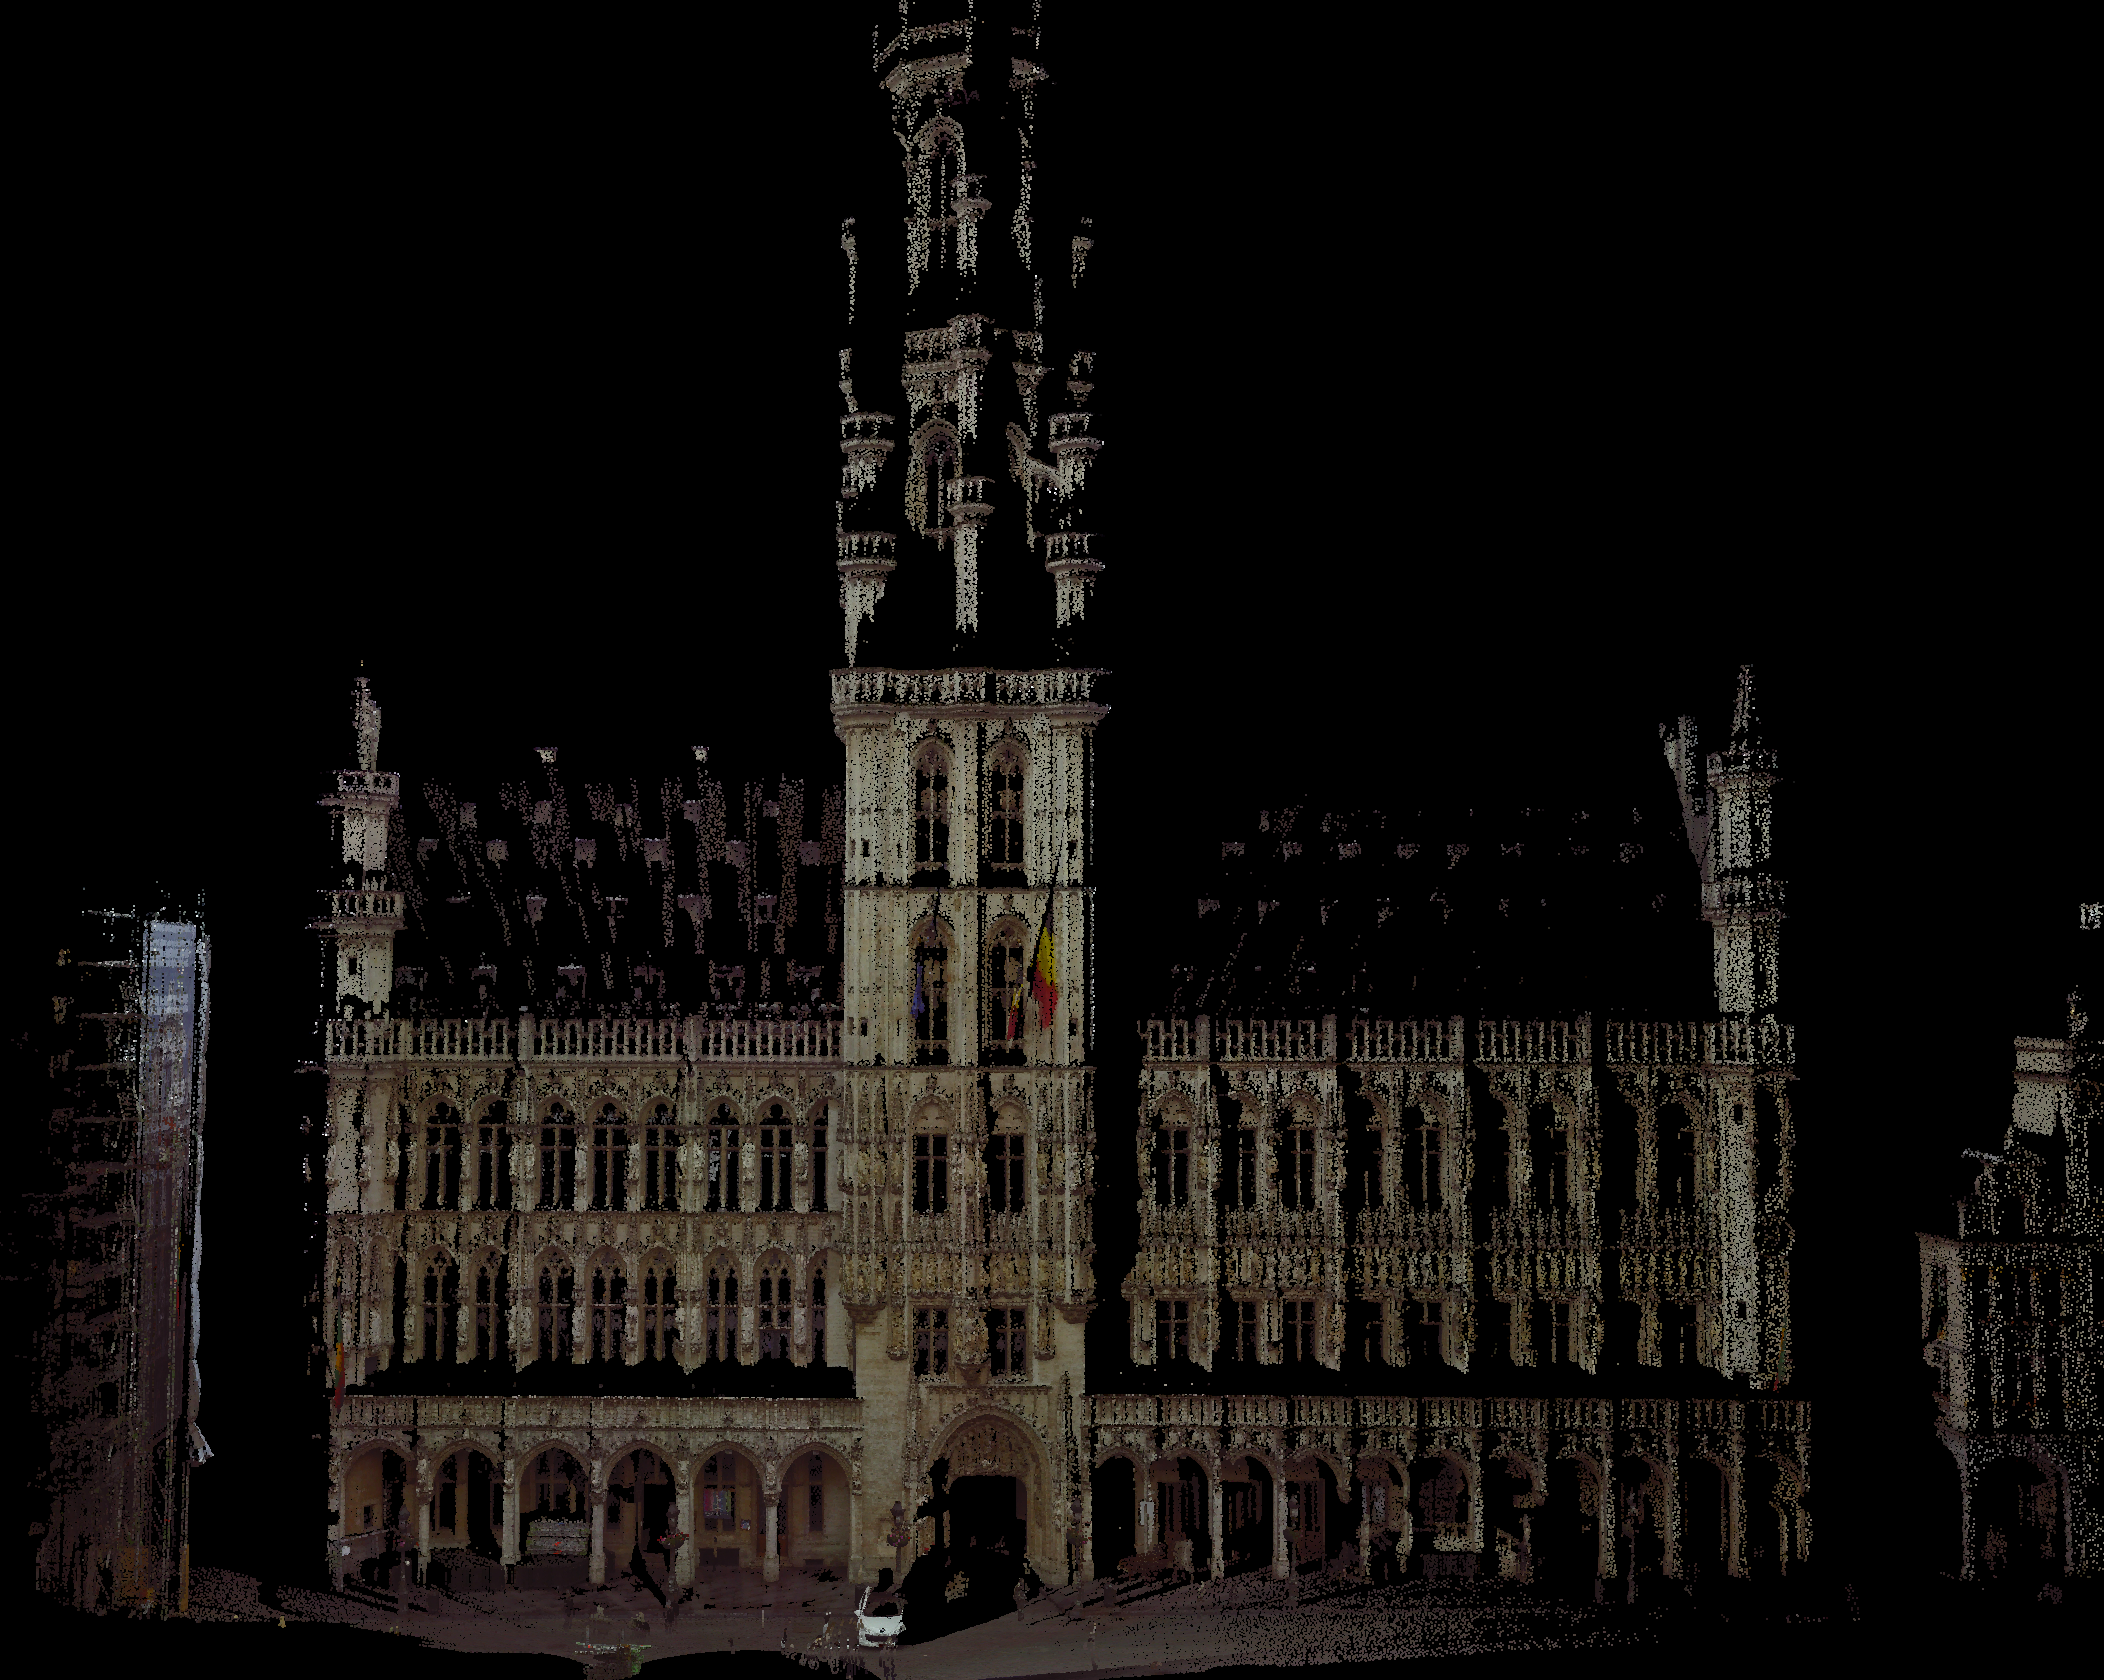
\includegraphics[width=\textwidth]{fig/scan_005.png}
\caption{Depiction of long range scan of Hôtel de Ville facade.}
\label{fig:scan_005}
\end{figure}


\subsection{Dessus-de-porte}
For usage in testing high-to-low resolution registration, two scans from the ``dessus-de-porte'', the stone artwork located above the front gate of the building, are used. It can be seen from a distance on the long range scan \ref{fig:scan_005}. A much higher resolution, close range scan has also been taken of this part only, and is shown in figure \ref{fig:scan_012}.

\begin{figure}[h]
\centering
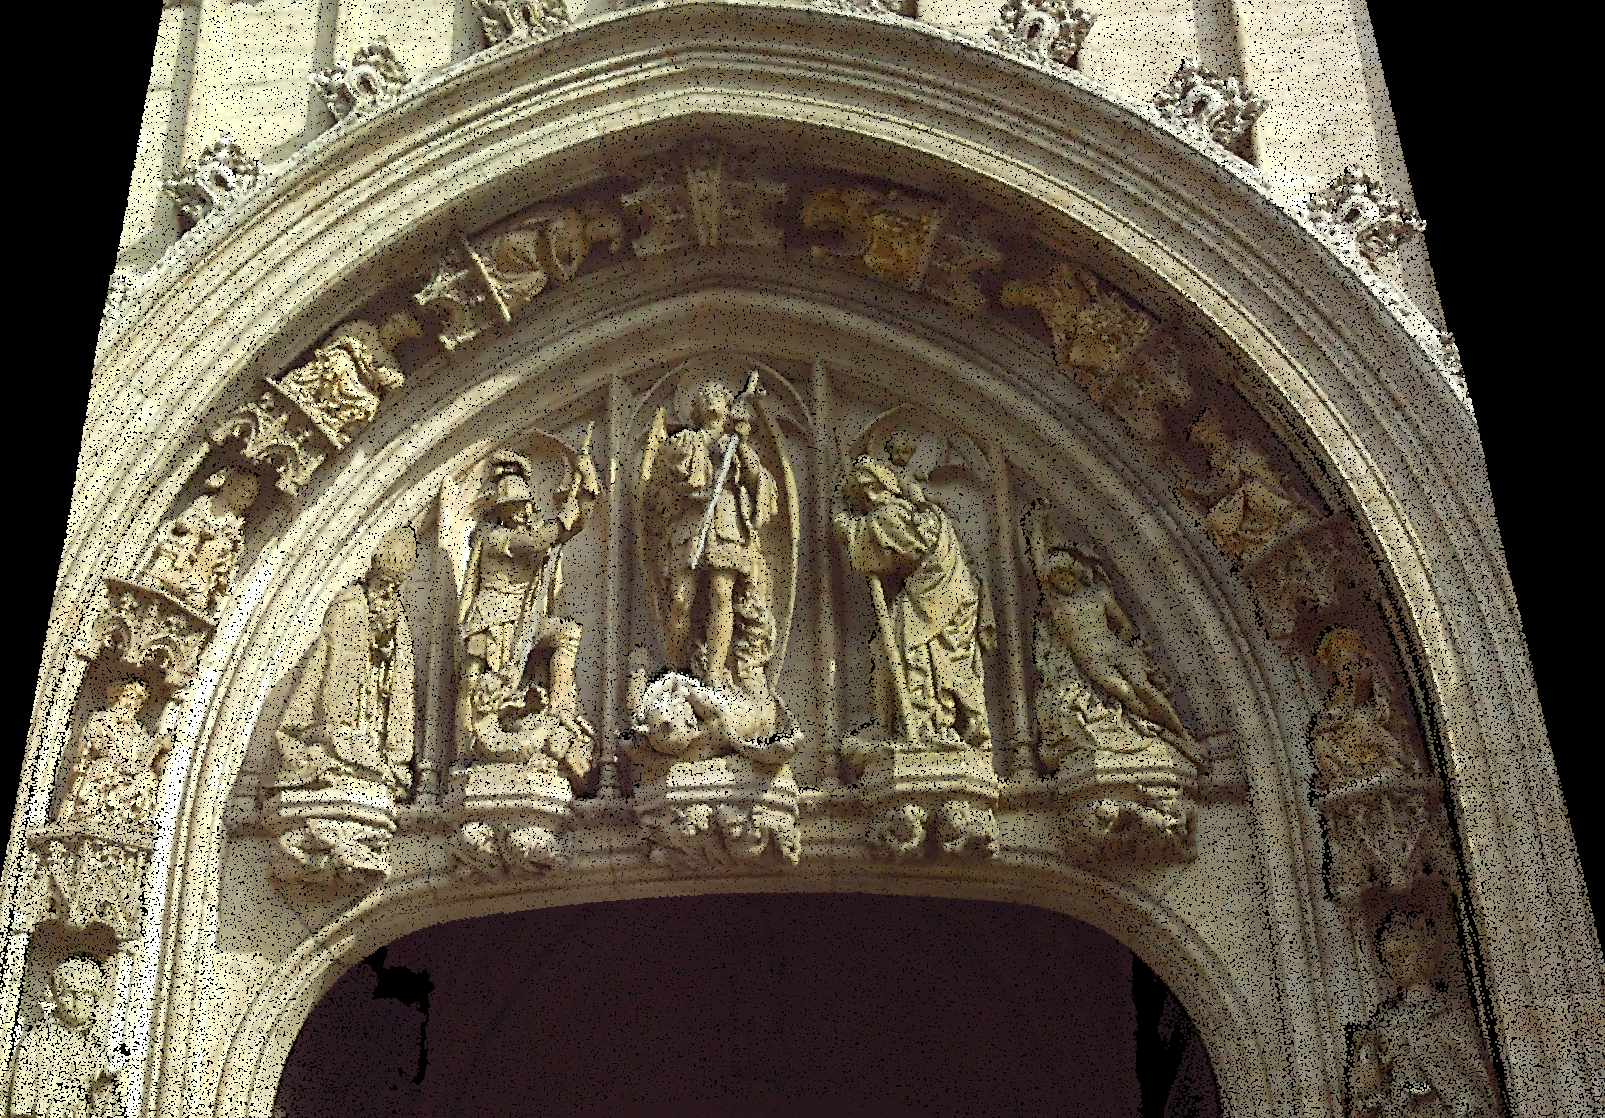
\includegraphics[width=.6\textwidth]{fig/scan_012.png}
\caption{Depiction of short range scan of dessus-de-porte facade.}
\label{fig:scan_012}
\end{figure}

As a 	first step of preprocessing, approximatively the same part has been cropped out of both scans, resulting in the two point clouds shown on figure \ref{fig:ddp_hilo}:

\begin{figure}[h]
\centering
\begin{subfigure}{.5\textwidth}
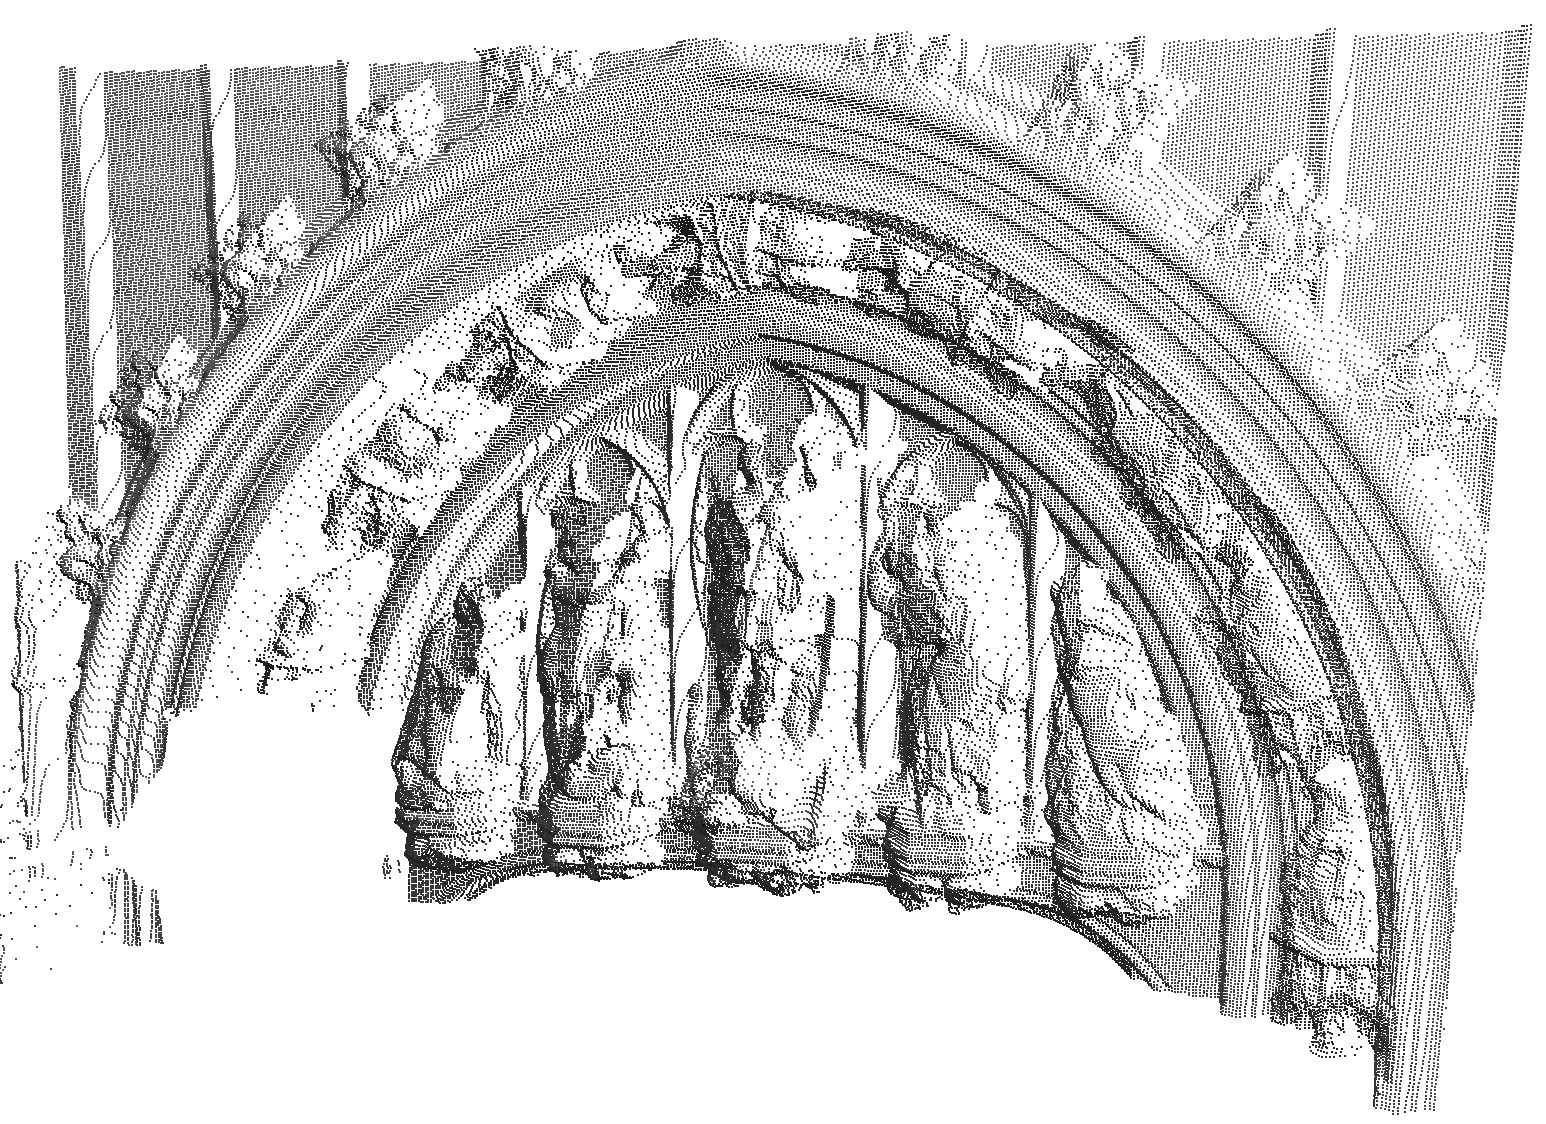
\includegraphics[width=\linewidth]{fig/ddp_LO.png}
\caption{Low-resolution}
\end{subfigure}%
\begin{subfigure}{.5\textwidth}
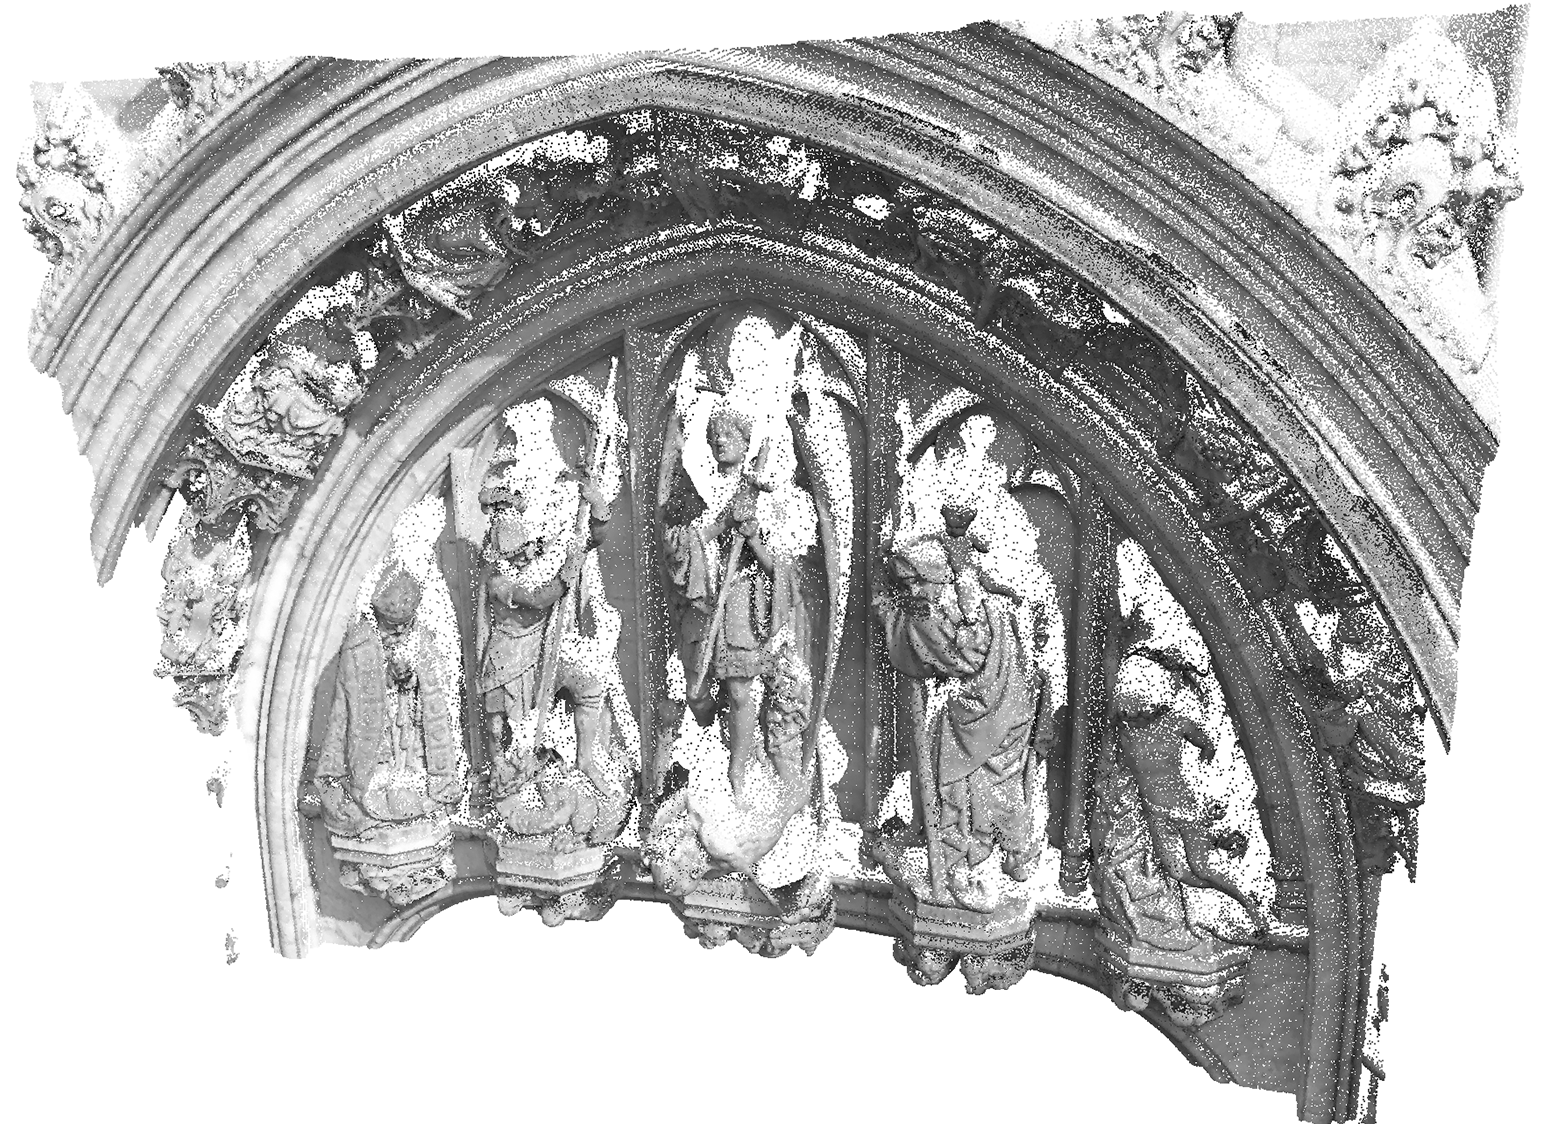
\includegraphics[width=\linewidth]{fig/ddp_HI.png}
\caption{High-resolution}
\end{subfigure}
\caption{Cropped scans of high and low resolution view of dessus-de-porte}
\label{fig:ddp_hilo}
\end{figure}

Colors have been removed on these depictions. The point clouds still have the color information, but it will not be used for registration. The point clouds also are still \emph{range images}, and information about the relative scanner poses is retained. It can be seen that the low resolution scan has a much lower point density. Its average distance between neighboring points, on flat surfaces facing the scanner, is about $10$ times higher than that of the high resolution scan. The high resolution scan depiction has been randomly downsampled as a side-effect of the visualization software. A close-up view of it is seen on figure \ref{fig:closeup_ddp}, later in this chapter. It can be seen that different sides of the sculptures are occluded in the two scans, because they have been recorded from different view points.

These point clouds have been manually coarsely aligned, and the surface normal vectors have been computed using an external software. A goal will be to finely register them, despite the differences in resolution.


\section{Relief point cloud} \label{sec:relief}
Many different kinds of objects can be scanned and good approaches for processing and registering them depend on many factors. To be able to study registration of point clouds, it is useful to generate artificial points clouds for which exact values of the underlying surface can be computed.

For this purpose an artificial point cloud class called ``relief'' point cloud will be described, which was designed to have similar properties than the dessus-de-porte. An algorithm was devised to generate relief surfaces. Figure \ref{fig:relief_render} shows a relief surface.

\begin{figure}[H]
\centering
\begin{subfigure}{.5\textwidth}
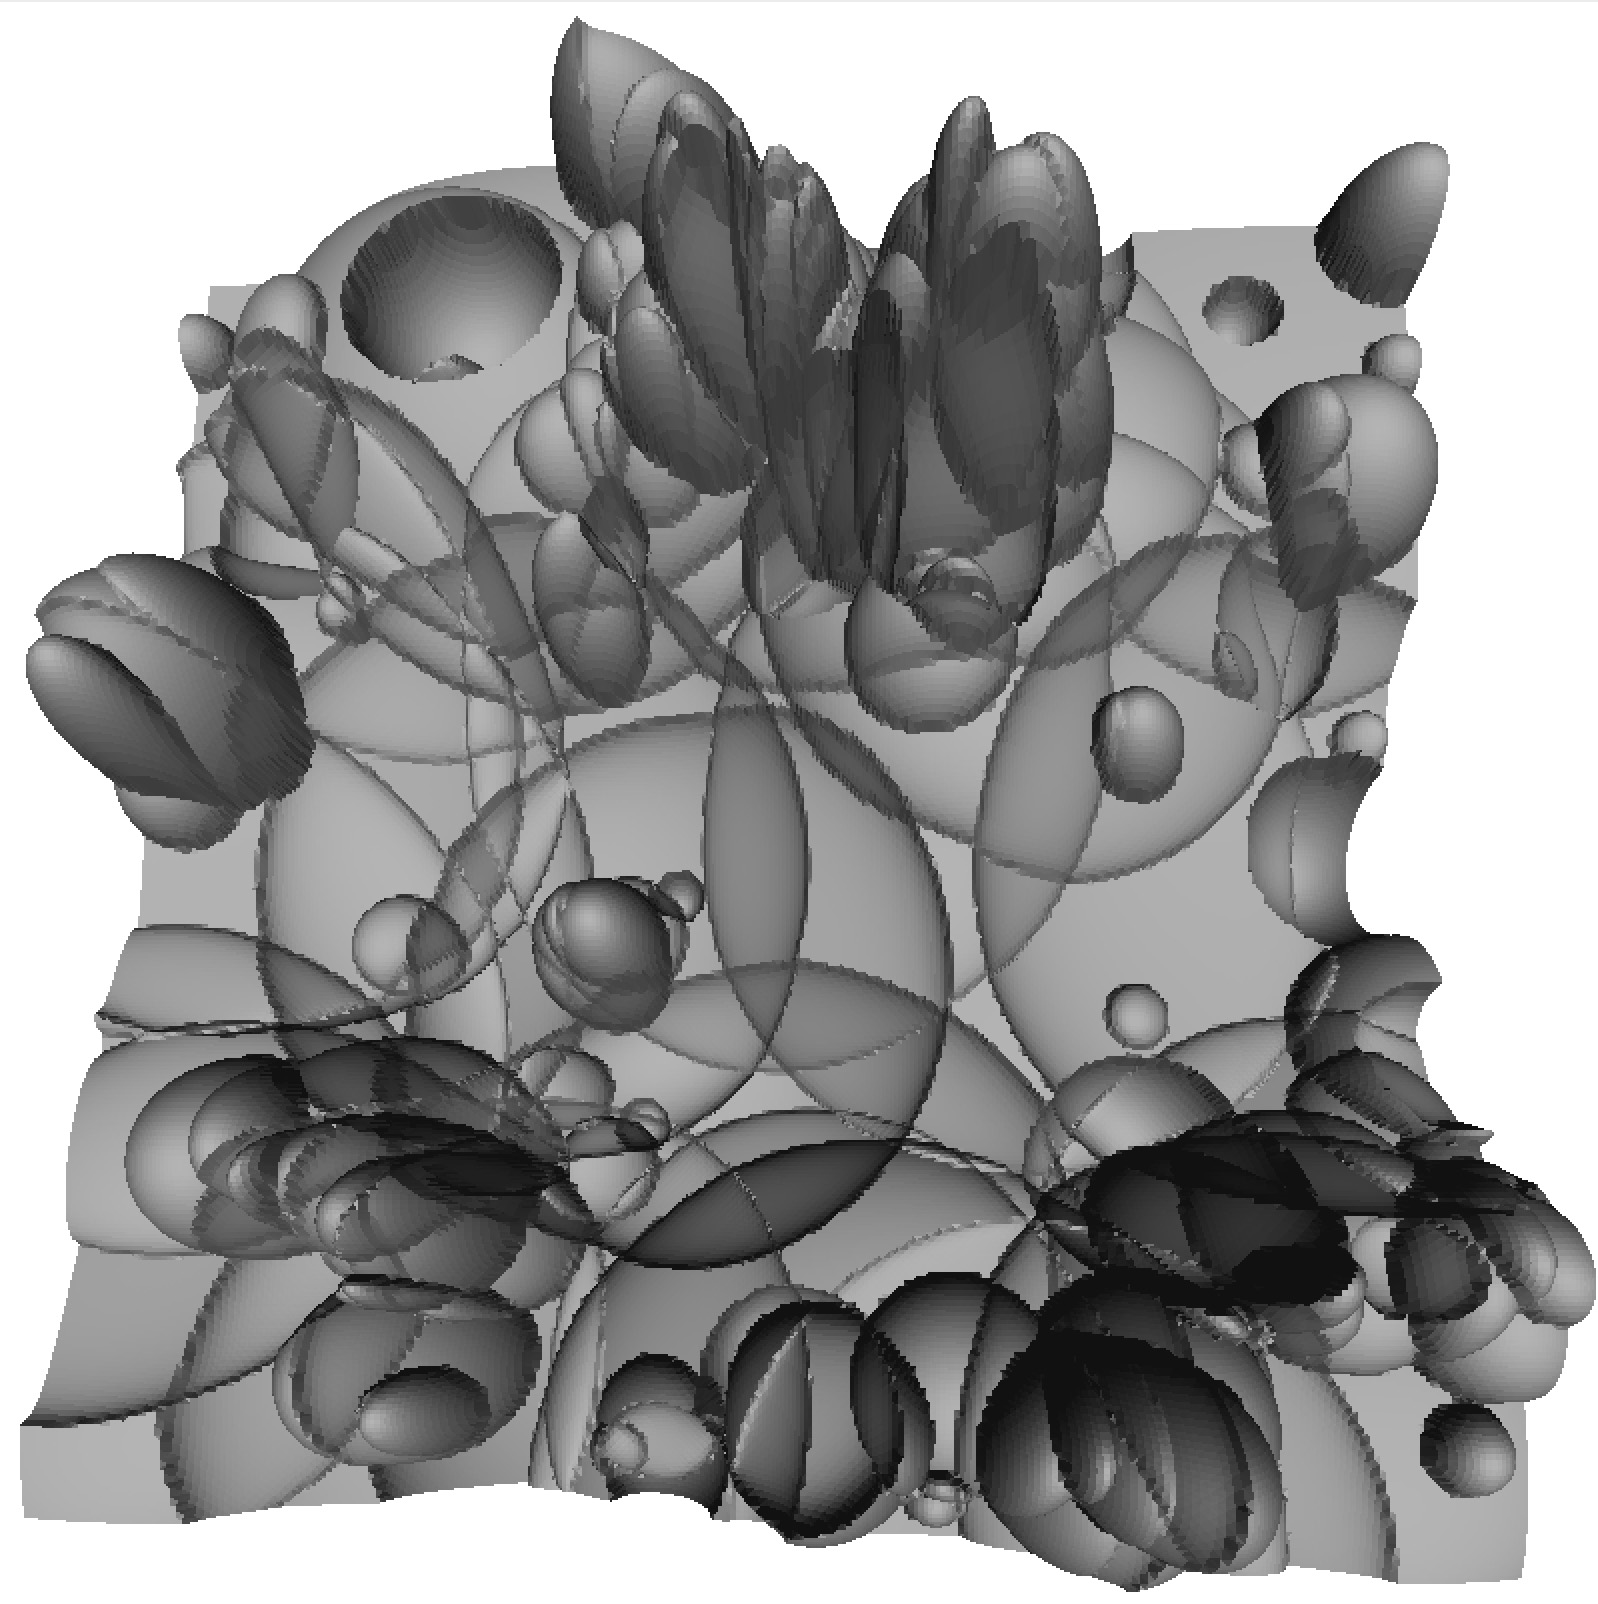
\includegraphics[width=\linewidth]{fig/r1_render2.jpg}
\end{subfigure}%
\begin{subfigure}{.5\textwidth}
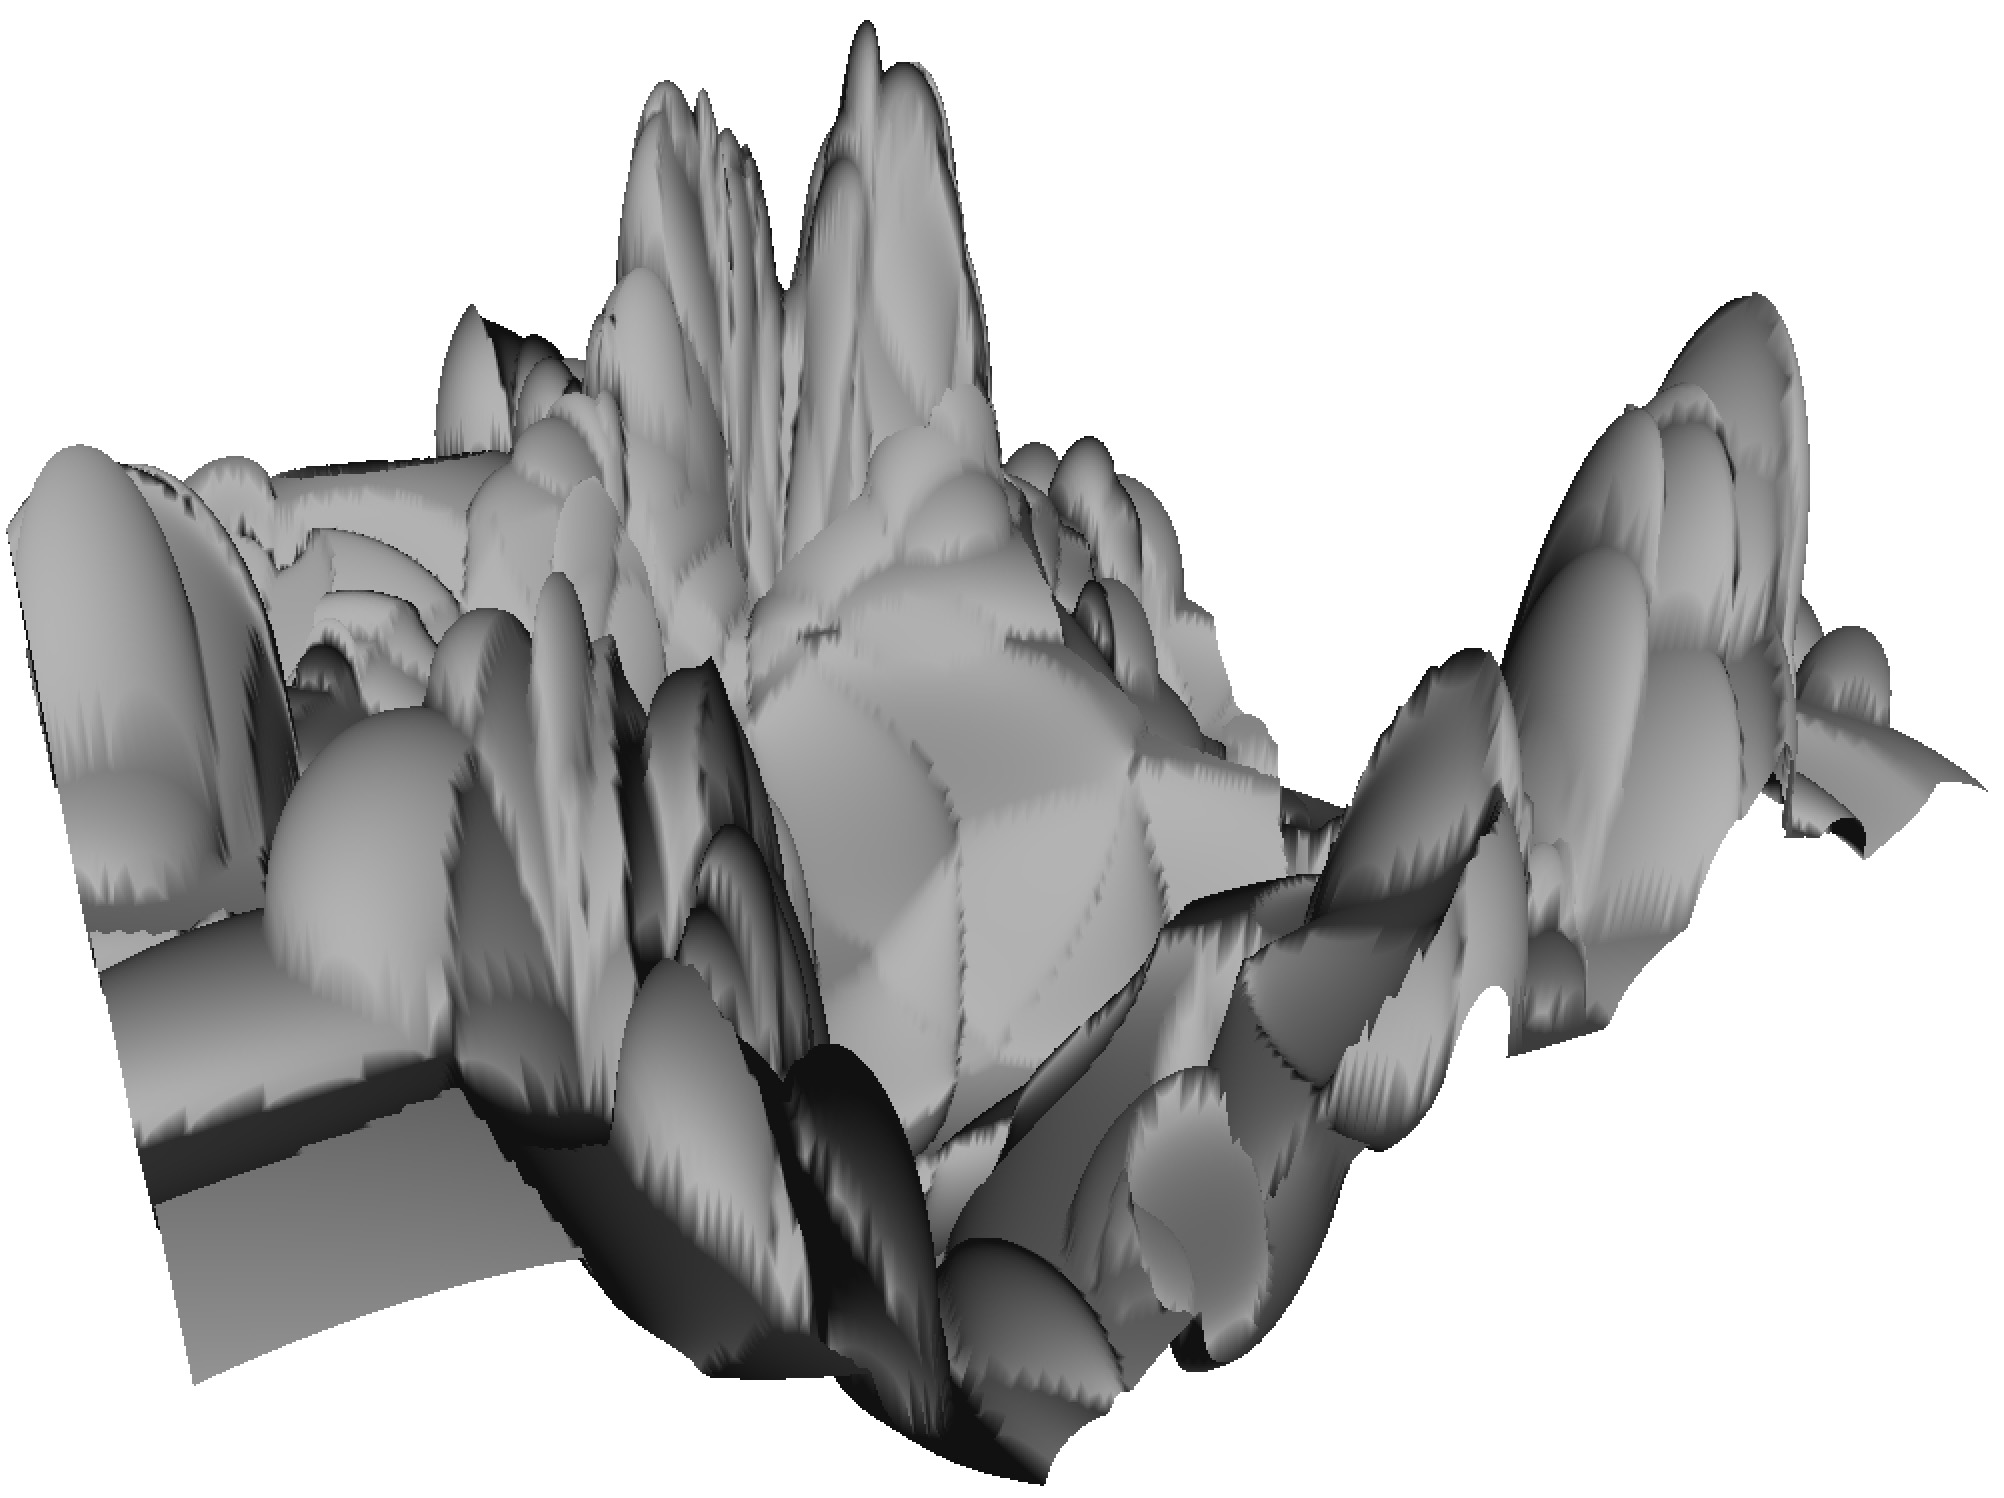
\includegraphics[width=\linewidth]{fig/r1_render1.jpg}
\end{subfigure}
\caption{Artificial relief surface, seen from two view points}
\label{fig:relief_render}
\end{figure}

The entire algorithm is randomized, but can be made deterministic by specifying a seed value for the random number generator. The surface to generate is specified by a \emph{width} $w$, a \emph{height multiplier} $h$, and this seed value.

The generated point cloud is a height map on the XY-plane. Let $z = R[x,y]$ be the $z$ component of the single point with given $x, y$ components. It is defined for $-\frac{w}{2} \leq x,y \leq +\frac{w}{2}$. At first, let $R[x,y] = 0$ for all these points. The result is a square surface of side length $w$.

The algorithm proceeds by pushing randomized ``embossings'' into the surface. The embossings are the shape of a half-sphere distorted in Z direction, and are described using the height map formula
\begin{equation}
B_i[x,y] = \pm \, h_i \sqrt{1 - \frac{(x_i - x)^2 + (y_i - y)^2}{r_i^2}}
\end{equation}
A plot of its two-dimensional analogue is shown in figure \ref{fig:relief_B}. $B_i[x,y]$ is set to $0$ for coordinates $x,y$ outside the domain, that is, for $x,y : (x_i - x)^2 + (y_i - y)^2 > r^2$. As a consequence a sharp circular corner is formed around the border.

\begin{figure}[h]
\centering
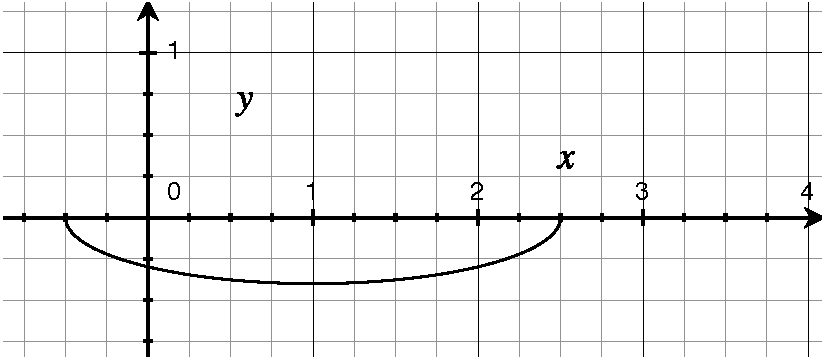
\includegraphics[width=.4\textwidth]{fig/relief_B.pdf}
\caption{2D example for relief embossing, with $h_i = -0.4$, $r_i = 1.5$, and $x_i = 1.0$}
\label{fig:relief_B}
\end{figure}

A fixed number $n$ of embossings $B_i$ are generated with different randomized parameters, and are added to $R$, so that
\begin{equation}
R[x,y] = \sum_{i=1}{n} B_i[x,y]
\end{equation}

The resulting height map will be split into regions $\{(x,y)\}$ where different subsets of $\{B_i\}$ are active. ($B_i$ is active when $(x,y)$ lies in its domain). $R$ has sharp corners at the border points of all $B_i$. As soon as more than one embossing is active in one region, the $z$ coordinate becomes a sum of square roots, producing a complicated shape for both the continuous surface areas and the corners. Its partial derivatives can still easily be calculated analytically, which allows for accurate computation of normal vectors. 

The radius $r_i$, height $h_i$ and center $(x_i, y_i)$ are randomly chosen for each embossing $B_i$. $x_i, y_i$ have a uniform distribution in $[-\frac{w}{2}, +\frac{w}{2}]$. The parameters for choosing $r_i$ and $h_i$ are set in such a way that the resulting surface will contain both flat regions and ``spikes'', which occlude parts of the surface when viewed from the side. Importantly, $h_i$ can be both positive or negative.

\subsection{Top-down view point cloud}
Two ways of generating a point cloud of a relief surface are used. The simplest way is to simply take a set of points $\{ x, y, R[x,y] \}$. It results in a \emph{top-down} view of the surface, as seen by an orthogonal projective camera\footnote{aka parallel camera} looking in $-z$ direction. From that view point the model has no occluded surfaces. The $x, y$ coordinates are arranged on a square grid. Figure \ref{fig:relief_plain} shows an example of such a point cloud, itself projected with a perspective camera.

\begin{figure}[h]
\centering
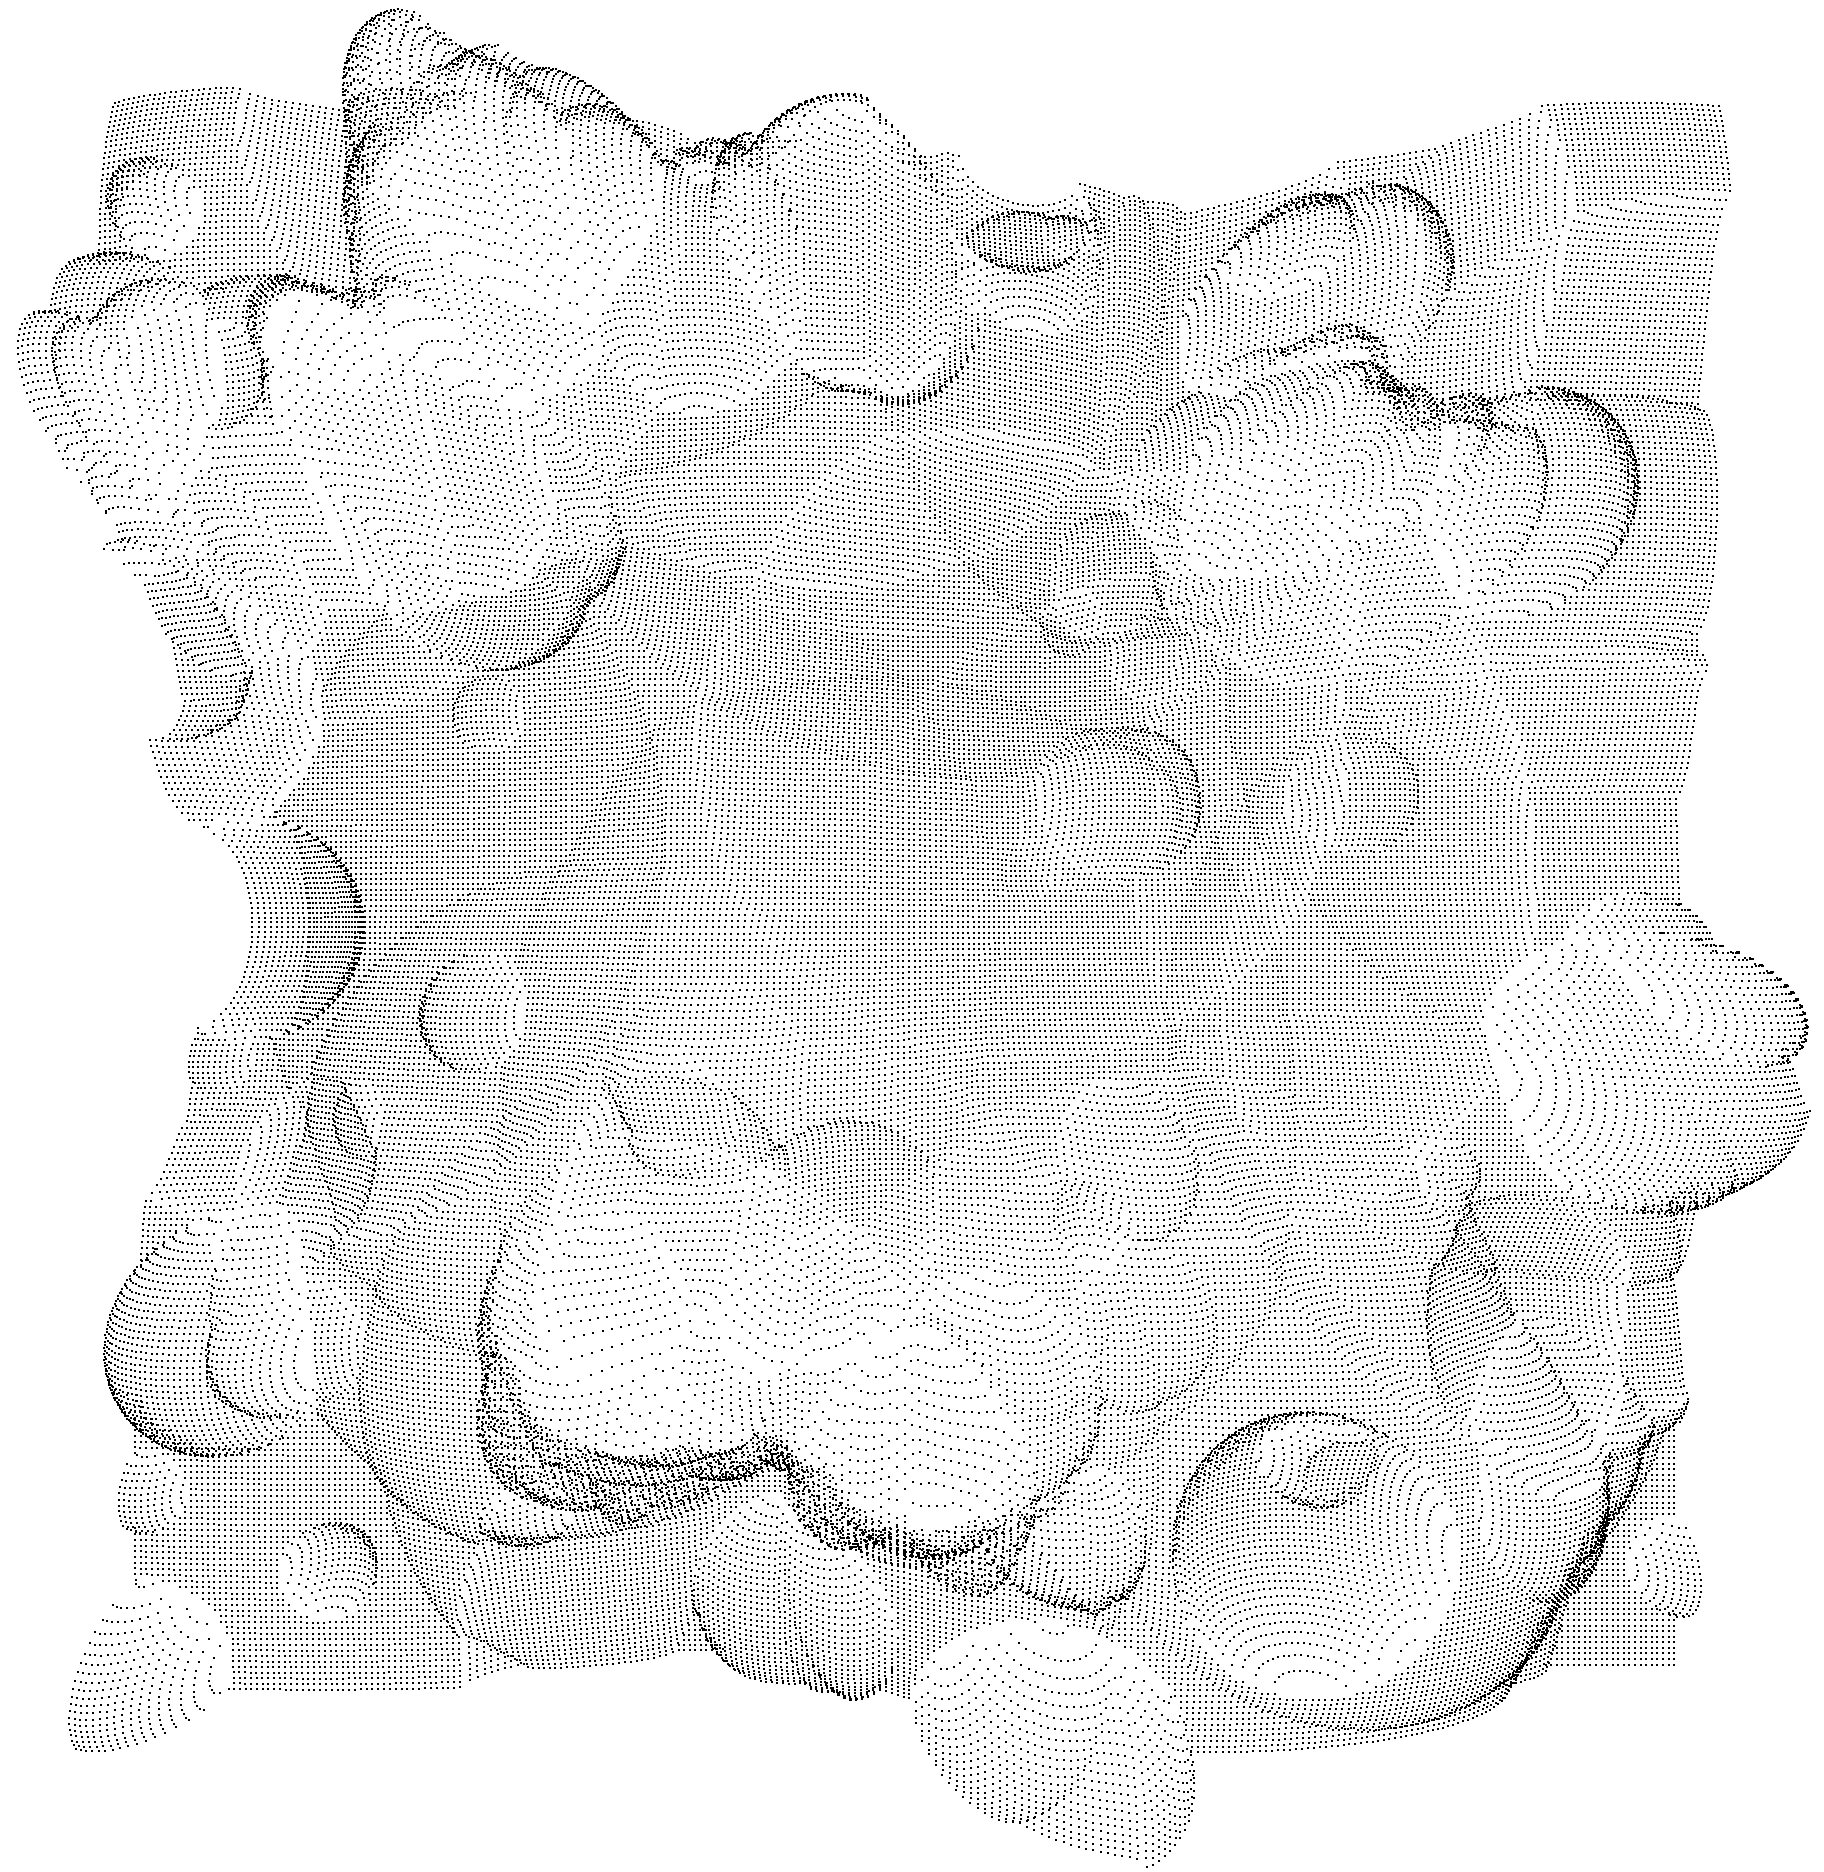
\includegraphics[width=.5\textwidth]{fig/r1_plain.png}
\caption{Top-down point cloud of relief}
\label{fig:relief_plain}
\end{figure}

\subsection{Occluded view point cloud}
However the goal of the artificial relief surface was to simulate the kinds of surfaces that occur on real objects, and to get a point cloud with similar properties as a 3D scan of it. So it is important to be able to generate point clouds of the relief as seen from other camera positions, with the occlusions that occur.

A virtual camera is placed near the surface at a given pose, and a range image is generated using it. With an orthogonal projection camera, the point density on the surfaces will remain constant, and with a perspective projection camera, it will decline with distance to the camera.

For the algorithm that creates this range image, an first attempt was to generate a top-down view point cloud with high enough density, and then project that point cloud into a range image as described in \ref{sec:pc_registration}. However, this inevitably leaves points in the occluded areas.

Another attempt was to implement a ray-tracing method that operates on the expression of $R[x,y]$: For each image pixel, calculate the intersections of the view ray with the surface $R$, and take the closest one. However, these intersections cannot easily be calculated analytically. Firstly, the various regions of $R$ with different active embossings must be considered separately. But even on a single such region, multiple intersection points can still occur, and there is no direct closed-form expression for finding them. So a lot of combinatorics and numerical approximation would be required.

Instead, the implemented algorithm generates a mesh of the surface, projects a depth map of it onto image space, and then back-projects the image pixel coordinates into points. Figure \ref{fig:relief_occlusion} shows the resulting point cloud from two view points, the second one near the projection camera pose.

\begin{figure}[h]
\centering
\begin{subfigure}{.5\textwidth}
	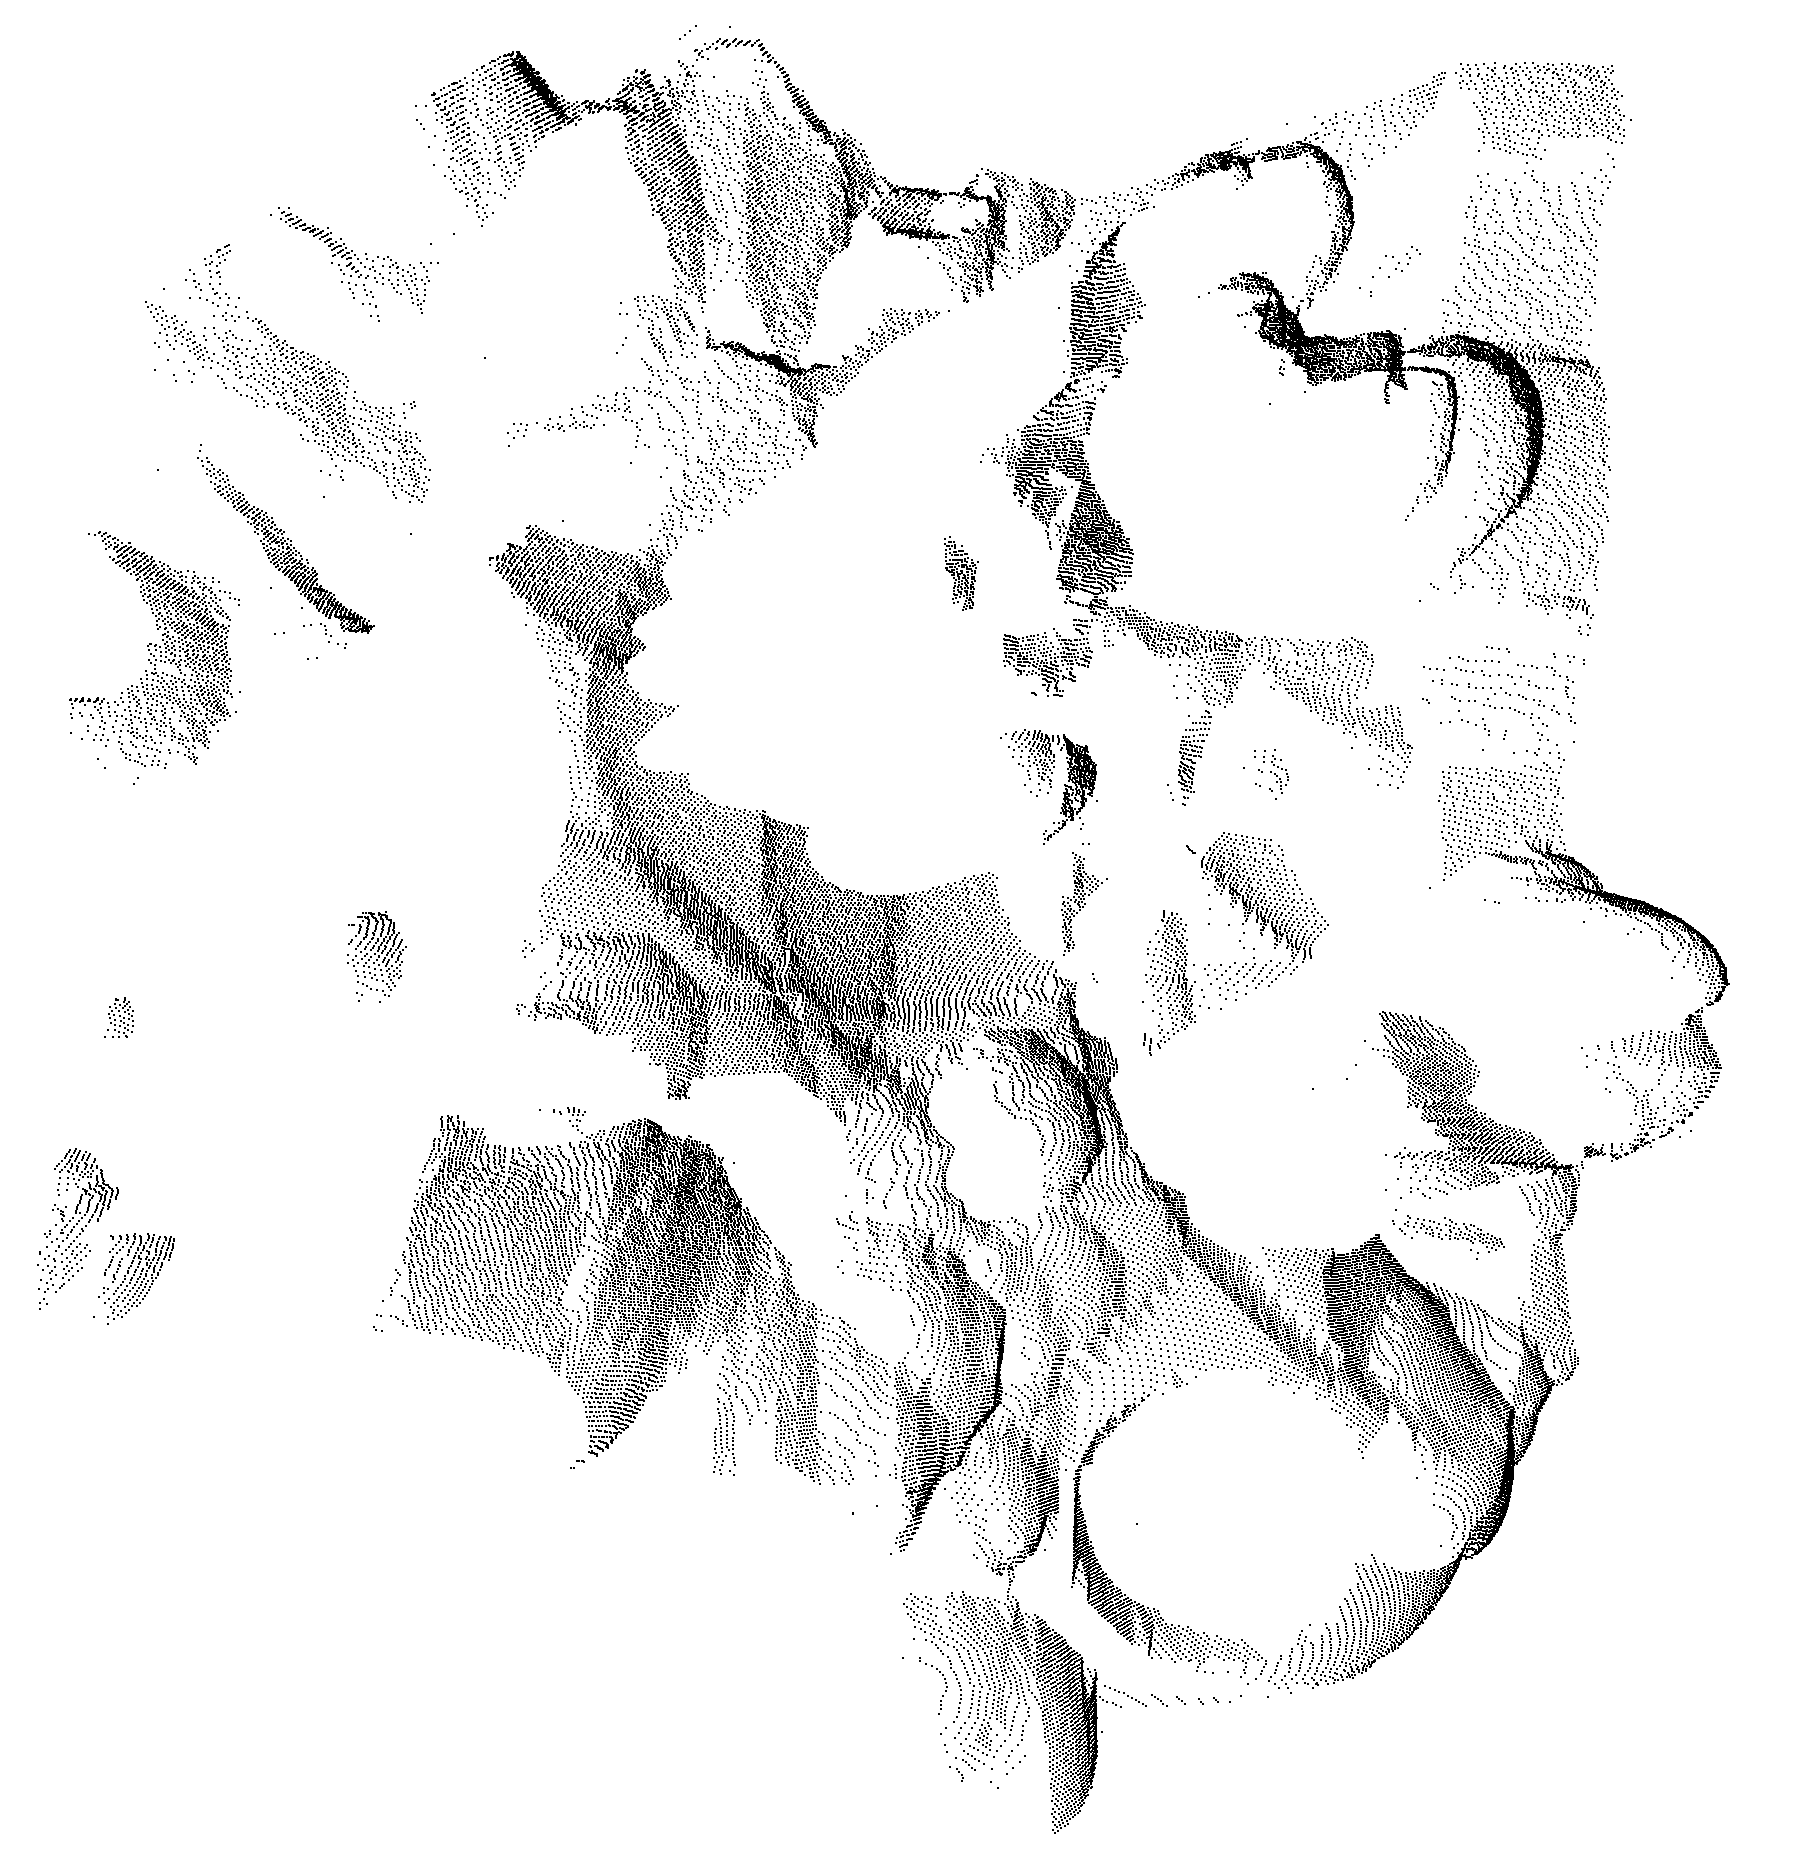
\includegraphics[width=\linewidth]{fig/r1_occlusion.png}
	\caption{Seen from above}
\end{subfigure}%
\begin{subfigure}{.5\textwidth}
	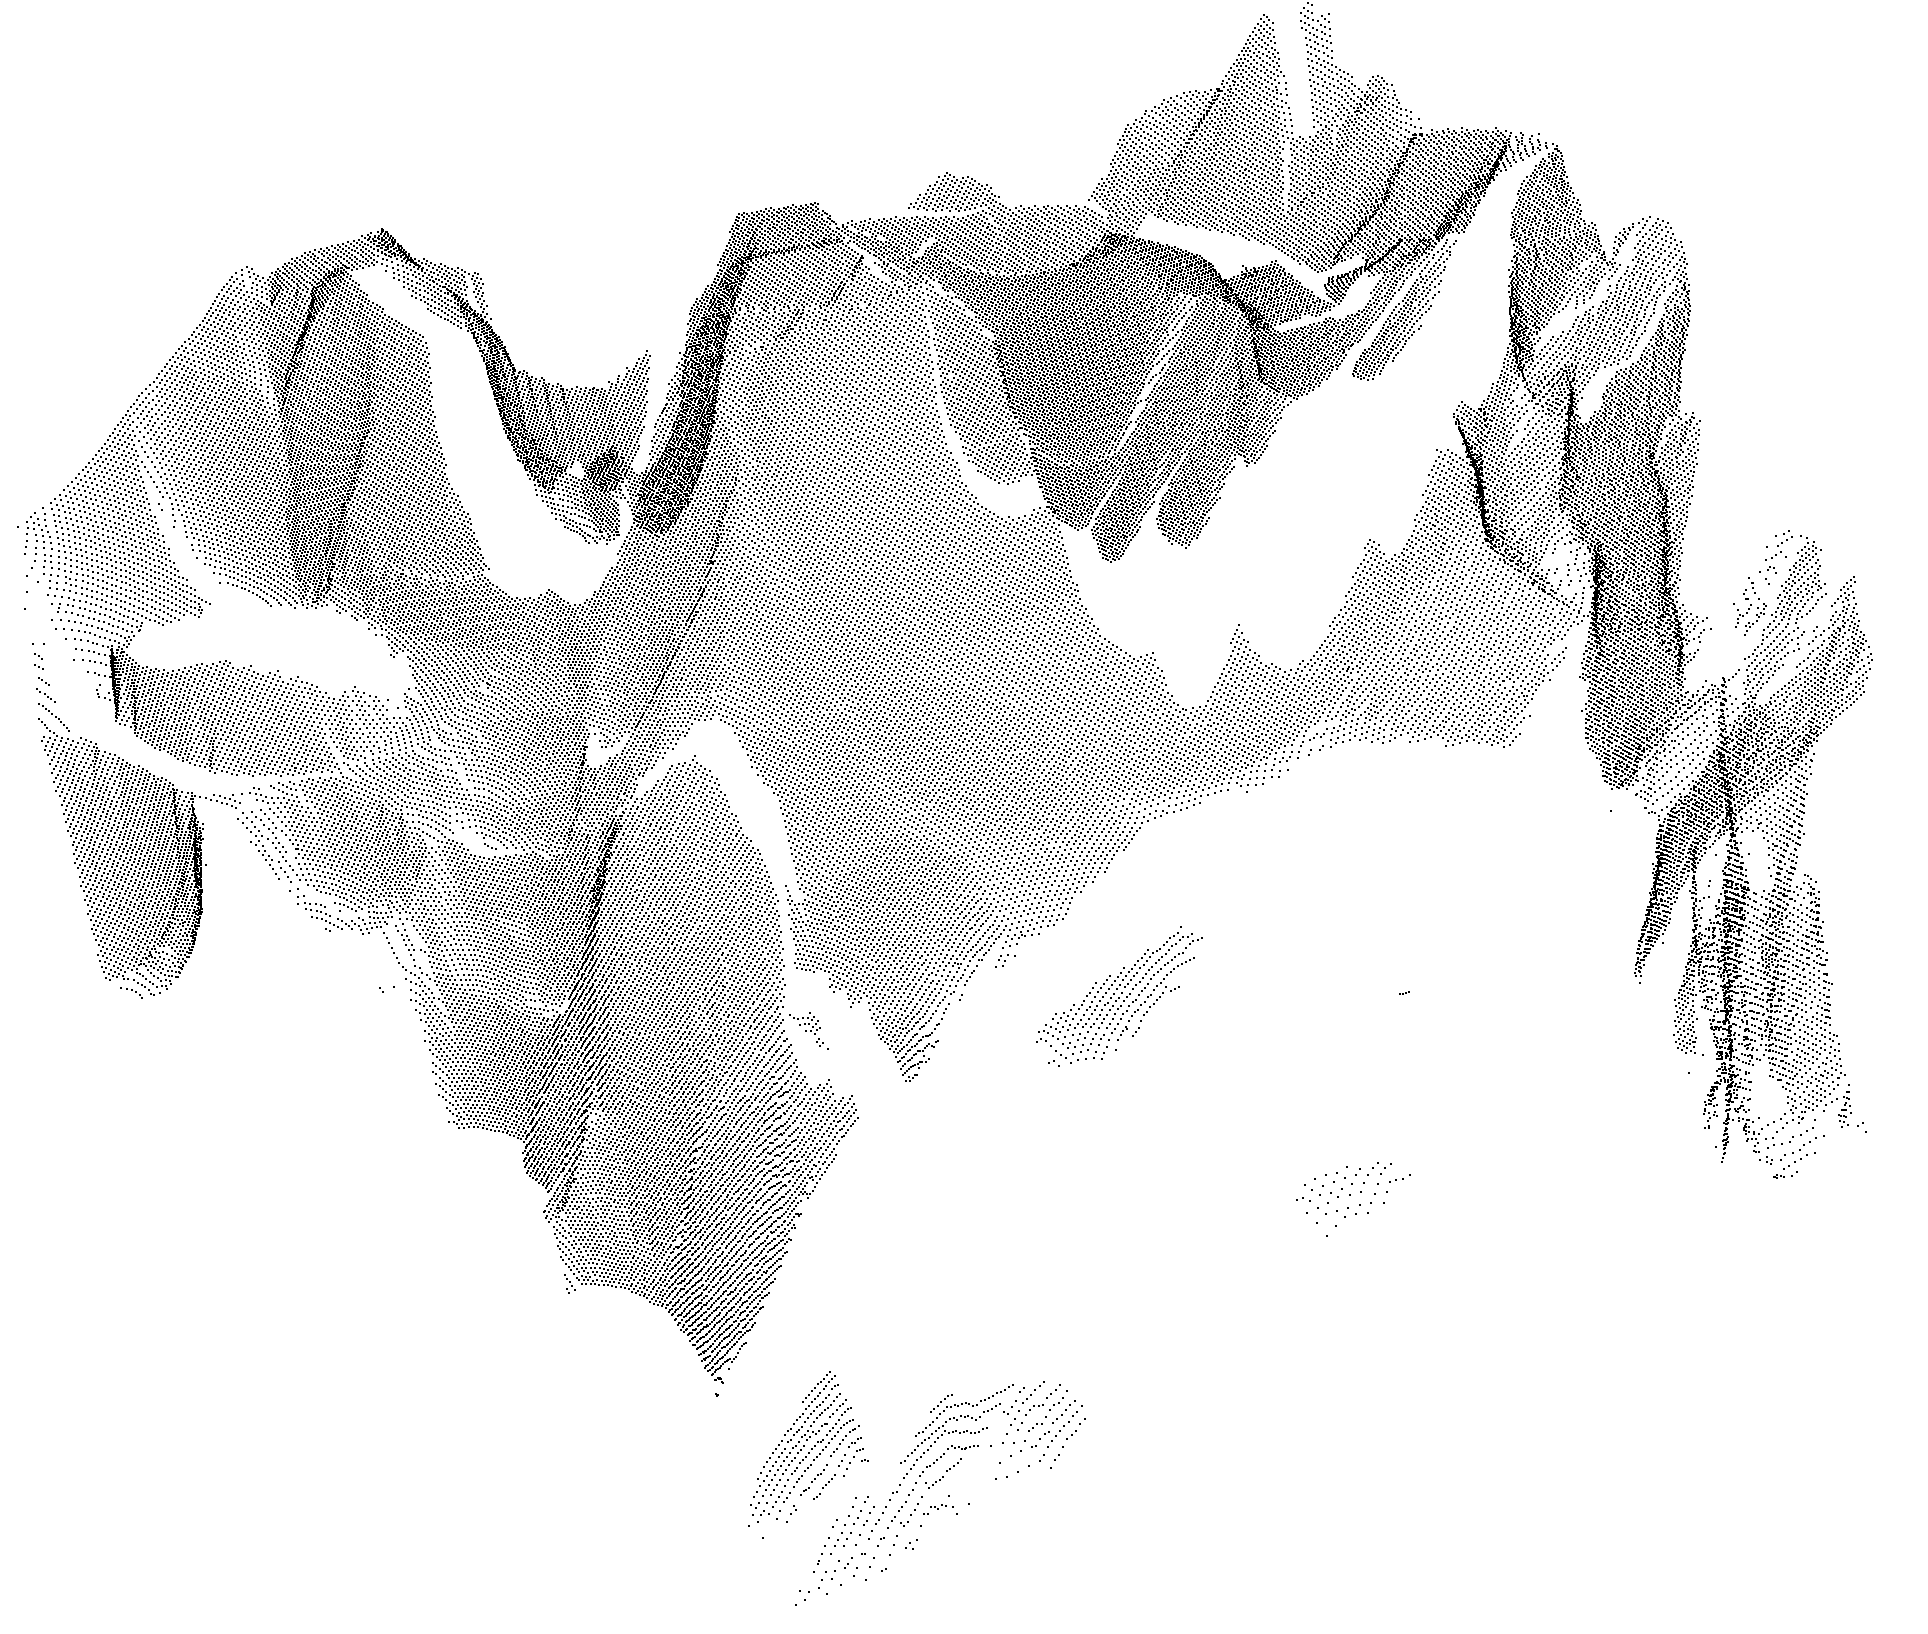
\includegraphics[width=\linewidth]{fig/r1_occlusion2.png}
	\caption{Seen from near the scanner's view point}
\end{subfigure}
\caption{Artificial relief surface point cloud with occlusion}
\label{fig:relief_occlusion}
\end{figure}

A triangle mesh is generated by taking points $\{ x, y, R[x,y] \}$ with the $(x,y)$ coordinates forming a square grid of a given density $\rho$, and adding a diagonal edge into each square, in alternating directions. The number of squares per side must be even for this. As can be seen on the renderings in figure \ref{fig:relief_render}, this mesh does not handle the sharp corners well, but it is sufficient as errors are rectified in a later step.

For each triangle, its three vertices are projected into image space, using the given projection camera. This image is a Z-buffer that contains, for each pixel, the inverted projected depth of the point\footnote{Z coordinate after application of camera projection matrix.}.

The width and height of this image space is set higher than that of the range image by a factor of about $k = 10$. Now each triangle is filled using a 2D rasterization algorithm. For each pixel, the inverted projected depths of the three corner points are linearly interpolated by using barycentric coordinates. This results in the inverted projected depth of the corresponding 3D surface point.

The actual occlusion culling is now done using a depth test: A pixel value is overwritten only if the inverse depth is higher than the previous one. This is the case only if the point is closer to the camera.

Each $k \times k$ square on this image corresponds to a pixel of the final range image. Its center pixel is taken. Given $(x_i, y_i)$ in image space, and the inverse projected depth of the surface point, the 3D coordinates $(x, y, z)$ of the surface points can now be calculated.

Due to the limited accuracy of the mesh, and floating point precision problems, there is some error in this result. It can be rectified by recalculating $z' = R[x, y]$.

\subsubsection{Alternate implementation}
Because the interpolation of the barycentric coordinates leads to an insufficient precision, an alternate approach has also been implemented: Along with Z-buffer, a second buffer is maintained in which every triangle is filled with a unique index value, with application of the depth test. In a separate list, each triangle index is associated with the four real numbers that define the plane spanned by the triangle $a x + b y + c z + d = 0$.

For the back-projection step, the intersection of the view ray and that plane is calculated.


\subsection{Similarity with dessus-de-porte}
Figure \ref{fig:relief_crop} (called $R$) shows an artificial relief point cloud with occluded view and additionally cropped to a random polygonal region inside the original square. It is superimposed on a top-down point cloud of the same relief.

It is similar to the dessus-de-porte point cloud (called $D$) in these ways:
\begin{itemize}
\item Approximatively planar. For $R$ the plane is the XY-plane, for $D$ it is the stone surface behind the five statues.
\item Seen from a side angle and partially occluded.
\item Contain smooth surfaces, sharp corners, and more complex areas.
\item Some near-planar surfaces, such as non-embossed areas in $R$, and the background stone surface in $D$.
\item Points dispersed on a regular lattice, as a result of the scan-lines, or of the image space in the virtual projection camera.
\end{itemize}

The important difference is that the underlying surface behind $R$ is known. The goal will be to develop a registration method that works for both $R$ and $D$ because of their common characteristics. On $R$ it can be tested both with and without knowledge of the surface.

\begin{figure}[h]
\centering
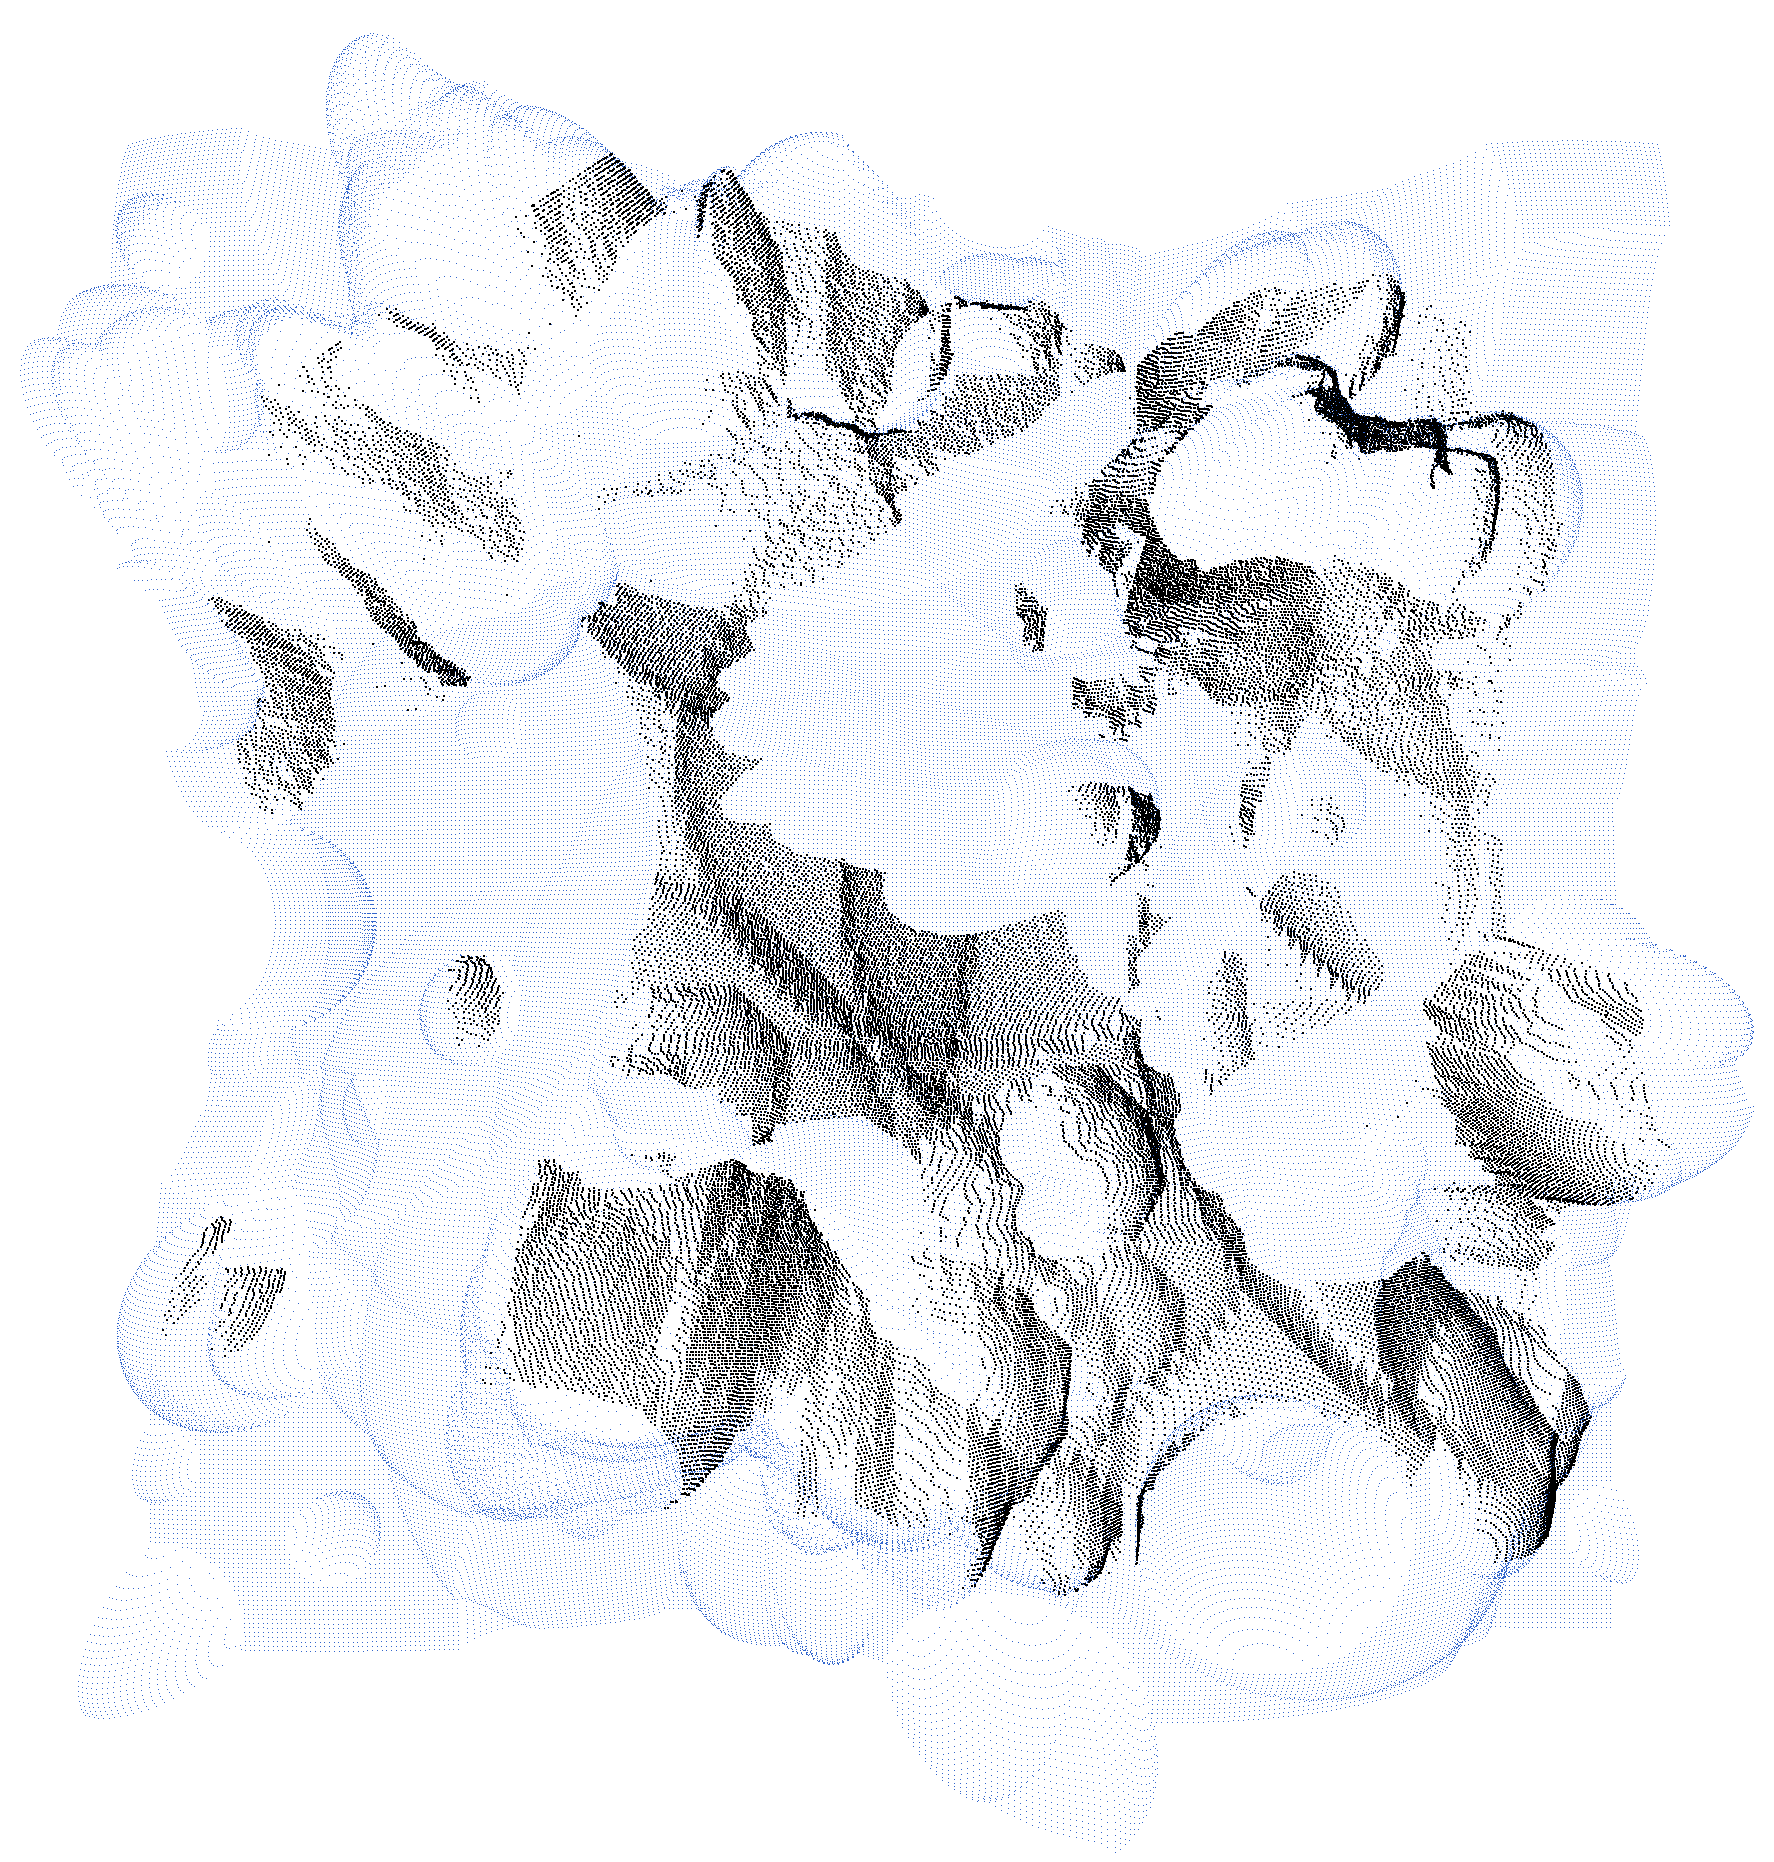
\includegraphics[width=0.5\textwidth]{fig/r1_crop.png}
\caption{$R$: Occluded view point cloud, and top-down point cloud of relief}
\label{fig:relief_crop}
\end{figure}


\section{Other models}
For the tests of the \gls{icp} algorithm, the well-known \emph{Stanford Bunny} model will also be used. This is a standard 3D test model used in computer graphics, available for free download along with other similar models. It depicts a ceramic figurine of a rabbit and was generated in 1994 at Stanford University. Different versions of it exist, the one used here is a point cloud that has already been registered from different view point scans, and covers the entire surface. It consists of $35947$ points.

During this chapter, artificial point clouds consisting of a single plane, or of a sphere, are also used.
